% WP X: "WP name"
% Deliverable DX.Y: "Name of this deliverable"
%
% Editors: Name and Surname of the Editor
% List of Authors:
%

\documentclass{SmartReport}
\usepackage{url, rotating}

\usepackage{subfig}
\usepackage{color}
\usepackage{paralist}
\usepackage{tabularx}
\usepackage{arydshln}
\usepackage{longtable}
\usepackage{tabu}
\usepackage{booktabs}


\newcommand{\todo}[1]{\noindent{\textcolor{red}{[TODO: #1]}}}

\begin{document}
\wpnumber{4} \wptitle{Peer Modeling and Search}
\instshort{UH} \delnumber{4.3} \versionnumber{0.1}
\contribshort{UH}
\deltitle{First Version of the Peer Search in Smart Societies}
\delshorttitle{Peer Search} 
\delavail{PU}
\delstatus{D}	
\duedate{30/6/2014}
\deldate{\today}
\delowner{Daniele Miorandi}
\wpleader{Alethia Hume, UNITN}
\qualityassessor{\ldots}
\smartkeywords{peer manager, search, privacy, ranking}
\maketitle

\begin{smartcontributors}
%date & reviewer (individual)\\
%0.1 & 04/11/2014 & 
UH & Daniele Miorandi \\
\end{smartcontributors}

%define the abstract
\begin{smartabstract}
%\textcolor{red}{Executive summary: max 1 page, objectives of the deliverable, achievements and impact on the project as a whole.}

This deliverable reports the outcomes of the activities carried out in WP4 on the peer profiling schemas and the privacy-aware mechanisms defined for the Peer Manager (PM). In particular, it includes a detailed description of the implementation and integration into the project infrastructure as well as the definition of evaluation procedures. 
%The main focus of the reporting period was the identification of appropriate evaluation mechanisms and the definition of an evaluation plan that should be inline also with the overall project evaluation.
Another achievement described in the deliverable  %during this period of the Smart Society project 
is the definition and initial integration of the privacy-enhancing component of the PM (integration with PrimeLife Policy Language), which is a fundamental building block for managing the information of peers in a privacy-preserving manner. 

Content-wise, the deliverable presents:
%\begin{enumerate}
\begin{inparaenum}[\itshape (i)]
\item The mechanisms and implementation details for the profile schemas and the privacy-enhancing technologies used by the PM;
\item The mechanisms and implementation details for the services that allow searching, matching and ranking of peers based on different attributes (i.e., characteristics) from their profiles;
\item The evaluation plans for WP4 including analytical and user-based evaluations; and
\item The description of how the PM is currently integrated in the SmartSociety platform and used in different project-wide scenarios.
\end{inparaenum}
%\end{enumerate}

%It is important to note also that while an evaluation plan is presented in this document, the actual evaluation and therefore the implementation of such plan will start during the second half of year 3 and will be formally reported as part of deliverable D4.4.
\end{smartabstract}


\section*{List of Acronyms}
\begin{tabular}{|c|p{3cm}|p{10cm}|}
\hline 
\textbf{Acronym} & \textbf{Full Name} & \textbf{Description} \\
\hline 
\hline 
%EC & Evaluator Component & System component in charge of evaluating the outcomes of each computation task (Sec.~\ref{sec:evaluator}).\\
%\hline 
CM & Context Manager & System componet in charge of monitoring the
context the agent represented on the platform by a peer is in.\\
\hline
IM & Incentives Manager & System component in charge of managing the implementation of incentive schemes.\\  
\hline 
KB & Knowledge Base &  System component in charge of storing and managing the knowledge in the platform.\\
\hline
OM & Orchestration Manager &  System component in charge of
orchestrating the lifecycle of tasks on the SmartSociety platform. \\
\hline 
PF & Programming Framework &  System component in charge of exposing
appropriate primitives and interfaces to application developers.\\
\hline 
PM & Peer Manager &  System component in charge of managing peers.\\
\hline \\
PS & Provenance Store & System component in charge of logging actions performed by platform components and peers.\\
\hline
RM & Reputation Manager & System componet in charge of handling the reputation of any system resource, including peers. \\
\hline
SmartCom & Communication Middleware & System component in charge of managing
communication channels between the platform and the peers. \\
\hline
\end{tabular}

\newpage

%%%%%%%%%%%%%%%%%%%%%%%%%%%%%%%%%%%%%%%%%%%%%%%%%%%%%%%%%%%%%%%%%%%%%%%%%%%%%%%%%%%%%%%%%%%%%%%%%%%%%%%%%%%%%%%%%%%%%%%%
%%%%%%%%%%%%%%%%%%%%%%%%%%%%%%%%%%%%%%%%

\section{Introduction}
\label{sec:intro}
\ldots

%%%%%%%%%%%%%%%%%%%%%%%%%%%%%%%%%%%%%%%%
%%%%%%%%%%%%%%%%%%%%%%%%%%%%%%%%%%%%%%%%%%%%%%%%%%%%%%%%%%%%%%%%%%%%%%%%%%%%%%%%%%%%%%%%%%%%%%%%%%%%%%%%%%%%%%%%%%%%%%%%
\newpage


%%%%%%%%%%%%%%%%%%%%%%%%%%%%%%%%%%%%%%%%%%%%%%%%%%%%%%%%%%%%%%
\section{Profiling}
\label{sec:profiling}
%\todo{RONALD - first draft by 30/May}

The \emph{Peer Manager (PM)} is a fundamental building block of the SmartSociety platform, providing a peer-centered data store that maintains and manages information about human- or machine-based peers within a privacy-preserving framework. 

\subsection{Mechanisms and algorithms}
%\todo{Peer Manager Theory - including flow diagram, pseudo-code if needed, whatever explain how it works}

The PM was designed as an extension of existing identity management systems, with the objective of keeping the information owned by peers private.
In order to provide a flexible management of information, the PM builds upon the notion of an \emph{entity-centric semantic enhanced model} that defines an extensible set of entity schemas providing the templates for an attribute-based representation of peers' characteristics~\cite{Giunchiglia_fromknowledge}. Additionally, the PM defines a \emph{storage and privacy protection model} by adding privacy regulations and considerations~\cite{Hartswood:2015fe}. 
The design of this model pays special attention to different privacy issues discussed by the Council of Europe in its recommendation {\sc{cm}}/{\sc{rec}}(2010)13 on profiling \cite{CoE2010}, as well as 
basic legal privacy principles enacted by the {\sc{eu}} Data Protection Directive 95/46/{\sc{ec}} \cite{EUDir95} and that affects profiles when they involve the storage and processing of personal data.

An important feature of the SmartSociety PM model is that the concrete meaning of schemas is further specified by mapping single elements (i.e., types of entities, the names of attributes and their values) to concepts from an underlying ontology that is also part of the same model~\cite{Giunchiglia_fromknowledge}. This design provides additional flexibility in the operations supported, allowing reasoning over peer's properties as well as the implementation of semantic-enhanced services.
%
The basic set of schemas/templates can be easily extended to support new application-specific scenarios requiring, for instance, the creation of new types of peers. The adaptability is provided by enabling the search and information sharing services to work over the new types in a way that is transparent to the rest of the HDA-CAS platform.

%%% Privacy%%%
A key feature of the PM is that the privacy of peers is protected by allowing people (i.e. users) to define profiles that contain and reveal only partial or (semantically) obfuscated information that is used for replying to information requests from other modules/components and is thus enforcing data minimisation. 
This allows, for example, a human peer to reveal whether it is a smoker and its age range (as a way to obfuscate the age and date of birth) when participating in a ride-sharing collective, while the same information can be hidden (i.e., completely obfuscated) when participating in a question-answering collective.

%%% Architecture %%%
The details about the internal architecture of the PM was presented in~\cite{D4.2,Hartswood:2015fe}, however, we recall one of its main component (i.e., the Peer Base) in the conceptual view shown in Figure~\ref{fig:peerManagerPlatform}. The Peer Base is composed of the following sub-components: 
\begin{itemize}
\item A \emph{Platform-Wide Knowledge Base} (${KB}_{PW}$) that stores the core entity types and the underlying ontology, allowing interoperability among SmartSociety components. 
\item A \emph{Platform-Wide Entity Base} (${EB}_{PW}$) that stores entity instances of general interests as well as public profiles of peers (i.e., information that each peer decides to publish in the platform about themselves).
\item A \emph{Knowledge Base} (${KB}_i$) and an \emph{Entity Base} (${EB}_i$) for each peer, which store the peer’s information. The peer maintains control over its data space and defines the privacy policies that apply to the data stored in it. 
%The peer's $KB$ is bootstrapped with the content of the platform-wide's $KB$, which then can be extended/specialized by the peer. The peer's $EB$ stores entity instances that are relevant to the peer (i.e., peer’s personal information, its resources, locations, roles, tasks, etc.). 
\end{itemize}
This storage separation for each of the peers and the platform is one of the Privacy-by-Design decisions taken by WP4 in accordance to the PM  privacy protection model.
%

\begin{figure}[t]
	\centering
	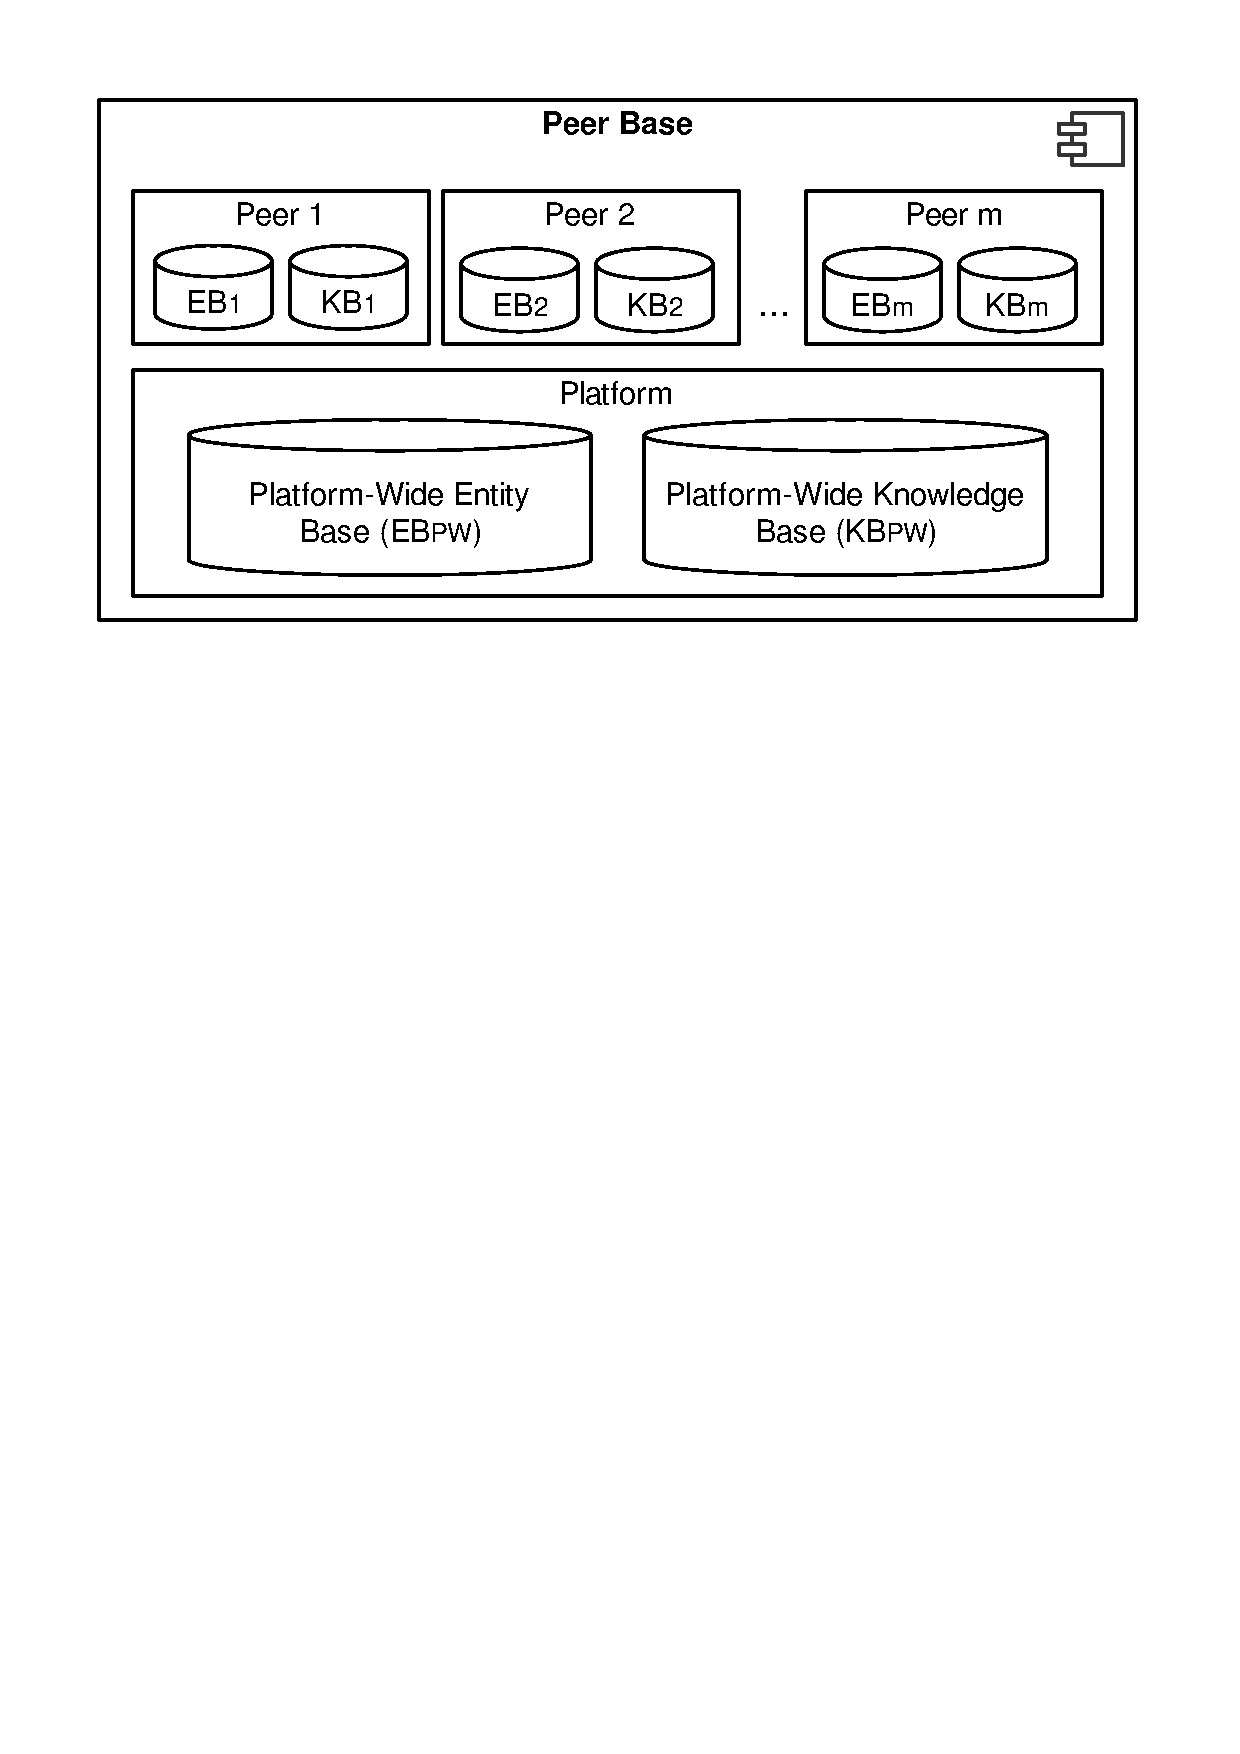
\includegraphics[width=0.65\linewidth]{figures/peerBase-diagram.pdf}
	\caption{Partial view of the Peer Manager internal architecture. Each subject its assigned its own peer storage, while the platform itself offers a shared Knowledge and Entity storages for different interactions.}
	\label{fig:peerManagerPlatform}
\end{figure}




\subsection{Implementation}
%{\it including how it has been implemented and specifications of APIs}

The Peer Manager component has been developed by following a three -layers approach, where each layer leverages the basic services offered by the level below and composes them for producing higher-level services. The resulting structure is shown in Figure~\ref{fig:pm-component-layers}; each layer will be further described in the remainder of this section. 

\begin{figure}[htbp]
\centering
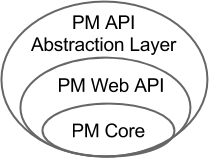
\includegraphics[width=0.3\textwidth]{figures/pm-component-layers.png}
\caption{Implementation layers of the Peer Manager}
\label{fig:pm-component-layers}
\end{figure}


\subsubsection{Peer Manager Core}
The Peer Manager Core provides a privacy-aware semantic storage for the SmartSociety Platform. This layer is implemented using Java, along with common data access frameworks like Spring and Hibernate.
While these technologies represent previous work from the University of Trento, the SmartSociety (through the work documented in~\cite{D1.1,D4.1,D4.2}) has created the Knowledge Model used for representing peers, users, profiles (i.e. personal information) and more generally managing the information for running an HDA-CAS.

No major changes have been done to the models or structures of the Peer Manager during the first half of Y-3 (so the research reported in previous deliverables still holds) but efforts to update these models to its final version will start in the second part of the year (as T1.4 restarts) and will have its results reported in Deliverable D1.3. No major changes are foreseen, so the underlying code and the exposed interfaces will likely be subject to minor revision only. 

\subsubsection{Peer Manager Web API} \label{ssec:pm-web-api}
This layer takes the Java classes that implement the Peer Manager Core and wraps them in HTTP API calls. 
No major changes to the APIs described in~\cite{D4.2} were introduced in Y-3. API specifications for this layer may be found in the Appendix~\ref{sec:pm-web-api-detail}.

\subsubsection{Peer Manager abstraction layer API} \label{ssec:pm-abs-api}
\todo{Content describing the purpose of this layer and the technologies used to implement it will be added to this section for the final version of this document}
 
This is a new component being developed specifically for the SmartSociety project and as such all code belonging to this layer will be open sourced. API Specifications for this layer may be found in the Appendix~\ref{sec:pm-abs-api-detail}.


\subsubsection{Integration with PPL policy language}
\todo{The content of this section needs to be refined}
\todo{Add a two-sentences description of what is PPL and its role in the overall PM functionality}
The integration process has been broken down in three incremental stages. 
% in three progressive steps or levels in order to better manage our development resources while complying with the SmartSociety project requirements.
%At each successive level both, the computational effectiveness of the achieved integration and the amount of work required, would increase. Nevertheless, the services offered by the integrated systems should remain mostly unchanged across the three levels of integration. 
\subsubsection{Basic Integration Approach - Decoupled Knowledge and Data}
\todo{Add A-PPL and Pii to the list of acronyms and define them}
In the first stage, for each of the profiles in the Peer Manager, A-PPL will have a corresponding Pii structure in its database. The overall structure is shown in Fig.~\ref{fig:pm-ppl-lv1.png}.

\begin{figure*}[htb!]
\centering
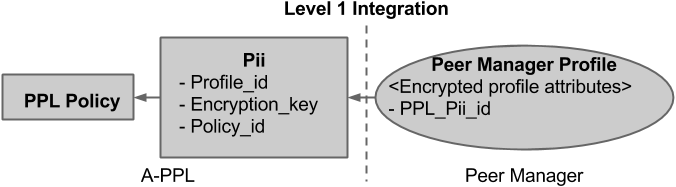
\includegraphics[width=0.8\linewidth]{figures/pm-ppl-lv1.png}
\caption{Basic Integration between the PM and PPL.}
\label{fig:pm-ppl-lv1.png}
\end{figure*}

It is important to note that the actual attribute information in the profile is not immediately accessible even to its owner (we may go as far as to encrypt it if necessary) and to read this information it needs to read the corresponding Pii entity stored in A-PPL (thus having to comply with the policy that protects the Pii).
\todo{Rephrase the next sentences and clarify what is *actually* delivered in the prototype}
Again, this is the simplest (but least effective way) to achieve integration and be absolutely sure that A-PPL authorizes the reading of the information in the Peer Manager Profile.
Of course there are issues to address, like having only a single unchanging encryption\_key for  each profile undermines purpose biding (you ask access to the info for one purpose and once granted access you can do whatever you want with the info, even use it for other purposes). Nevertheless, for Proof-of-Concept integration (and for this year's deliverable) I strongly believe this approach to be of enough value.

\subsubsection{Advanced Integration Approaches}
In the second stage of integration, the Peer Manager embeds knowledge of the inner details of PPL policies, so it is now able authorize the use of the information and store the information unencrypted, as shown in Fig.~{fig:pm-ppl-lv2.png}.

\begin{figure*}[htb!]
\centering
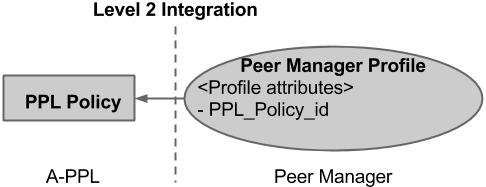
\includegraphics[width=0.6\linewidth]{figures/pm-ppl-lv2.png}
\caption{Advanced Integration between the PM and PPL.}
\label{fig:pm-ppl-lv2.png}
\end{figure*}

Note that the interaction with the A-PPL system is still used for the Policy storage (as the PM is supposed to have still no knowledge of how these policies are represented). Furthermore, the Peer Manager will still ask the A-PPL system if a requested operation complies or not with a given policy (as the PM does not share the same semantic ontology as A-PPL it cannot know if a request complies with a Policy even if it has all information about both structures).

In the final stage of integration the Peer Manager will represent a Policy as an Entity, and the A-PPL ontology used for reasoning about policies will be migrated to a specific and protected Knowledge Base in the Peer Manager.
With these two improvements, the Peer Manager will be able to support and enforce PPL without ever needing to call the A-PPL system. 


\subsubsection{Implementation of the Basic Integration Approach}
\todo{This is all in the future, so the Q is: what has actually been done so far?}
We will start with the level one integration, but in order to keep the generality we will make it possible to ask both about attributes and profiles. The profile will be treated as an ordinary attribute type. A profile is created for each purpose or combination of purposes needed.
In order to introduce the fact that an attribute is tied to one or more profiles and that encryption is needed the PIIType structure will be expanded with the fields profileID and encryptionData, encryption data in turn will consists of the fields  key, method and a list of parameters. Since no attribute type values are stored currently all attributes are considered to have a null value and the encrytionData is returned rather than the attribute value when the attribute type is retrieved.
In order to facilitate this the API of A-PPLE will be changed in the following way:
\begin{enumerate}
	\item We will add a structure containing profileID and encryption key in a many to one  relation to a PIITYPE. This will tie a list of profileID, encryptionData pairs to an attribute name and owner.
	\item We will construct a simpler version of the createPII call that do not require the sender to know about the PII type and also require profileID and encryptionData when storing and remove the attribute value since that is already stored in the PeerProfile.
	\item Since it can be cumbersome to make create calls for all attributes in a profile, if this should be needed we will violate the rest a bit and make a create call that takes a list of attributes and associated values and creates them in bulk. 
	\item We will change the getPII to require a profile id as well and to return encryptionData rather than the value of the attribute if it succeeds.
	\item  Like in 3 we will create a bulk call for retrieving multiple clearances and encryptionData for attribute names in bulk.
In the cases when just the profile attribute is used for clearance there we will have to need a ppl policy just containing the attribute name ”profile”, the profileID and the purpose covered by that profile. In order to do this the value (id) of that profile would have to be known when the policy is created so we would in have one specific policy for each profile. This ppl policy will however be fairly simple at the start and only differ in the profileID and purpose.
In order for A-PPLE and the Peer Manager to “understand” each other purpose names and attribute names needs to be aligned or known by both entities. 
\end{enumerate}

\section{Search, Matching and Ranking}
\label{sec:matching_ranking}
%\todo{ALETHIA - first draft by 30/May}

The search service provided by the Peer Manager (PM) was initially described in~\cite{D4.2}. In this deliverable we describe its evolution and provide more details about the meta-data models that are related with the search and ranking techniques, as well as their implementation.

\subsection{Mechanisms and algorithms}
%{\it including flow diagram, pseudo-code if needed, whatever explain how it works}

In order to select mechanisms and algorithms for implementing search in the PM we need to take into account existing approaches from the state of the art that can be used. For instance, there are many models and data structures that can be borrowed from the area of Information Retrieval (IR) as well as different matching techniques that can be used with different types of values. 

A logical view of the Search component is shown in Fig.~\ref{fig:search_diagram}, and presents the internal mechanisms, called subcomponents, that are integrated within the PM to deal with different types of queries (i.e., constraints on values of different natures). 
In what follows, these subcomponents are described in more details.

\begin{figure}[htbp]
\centering
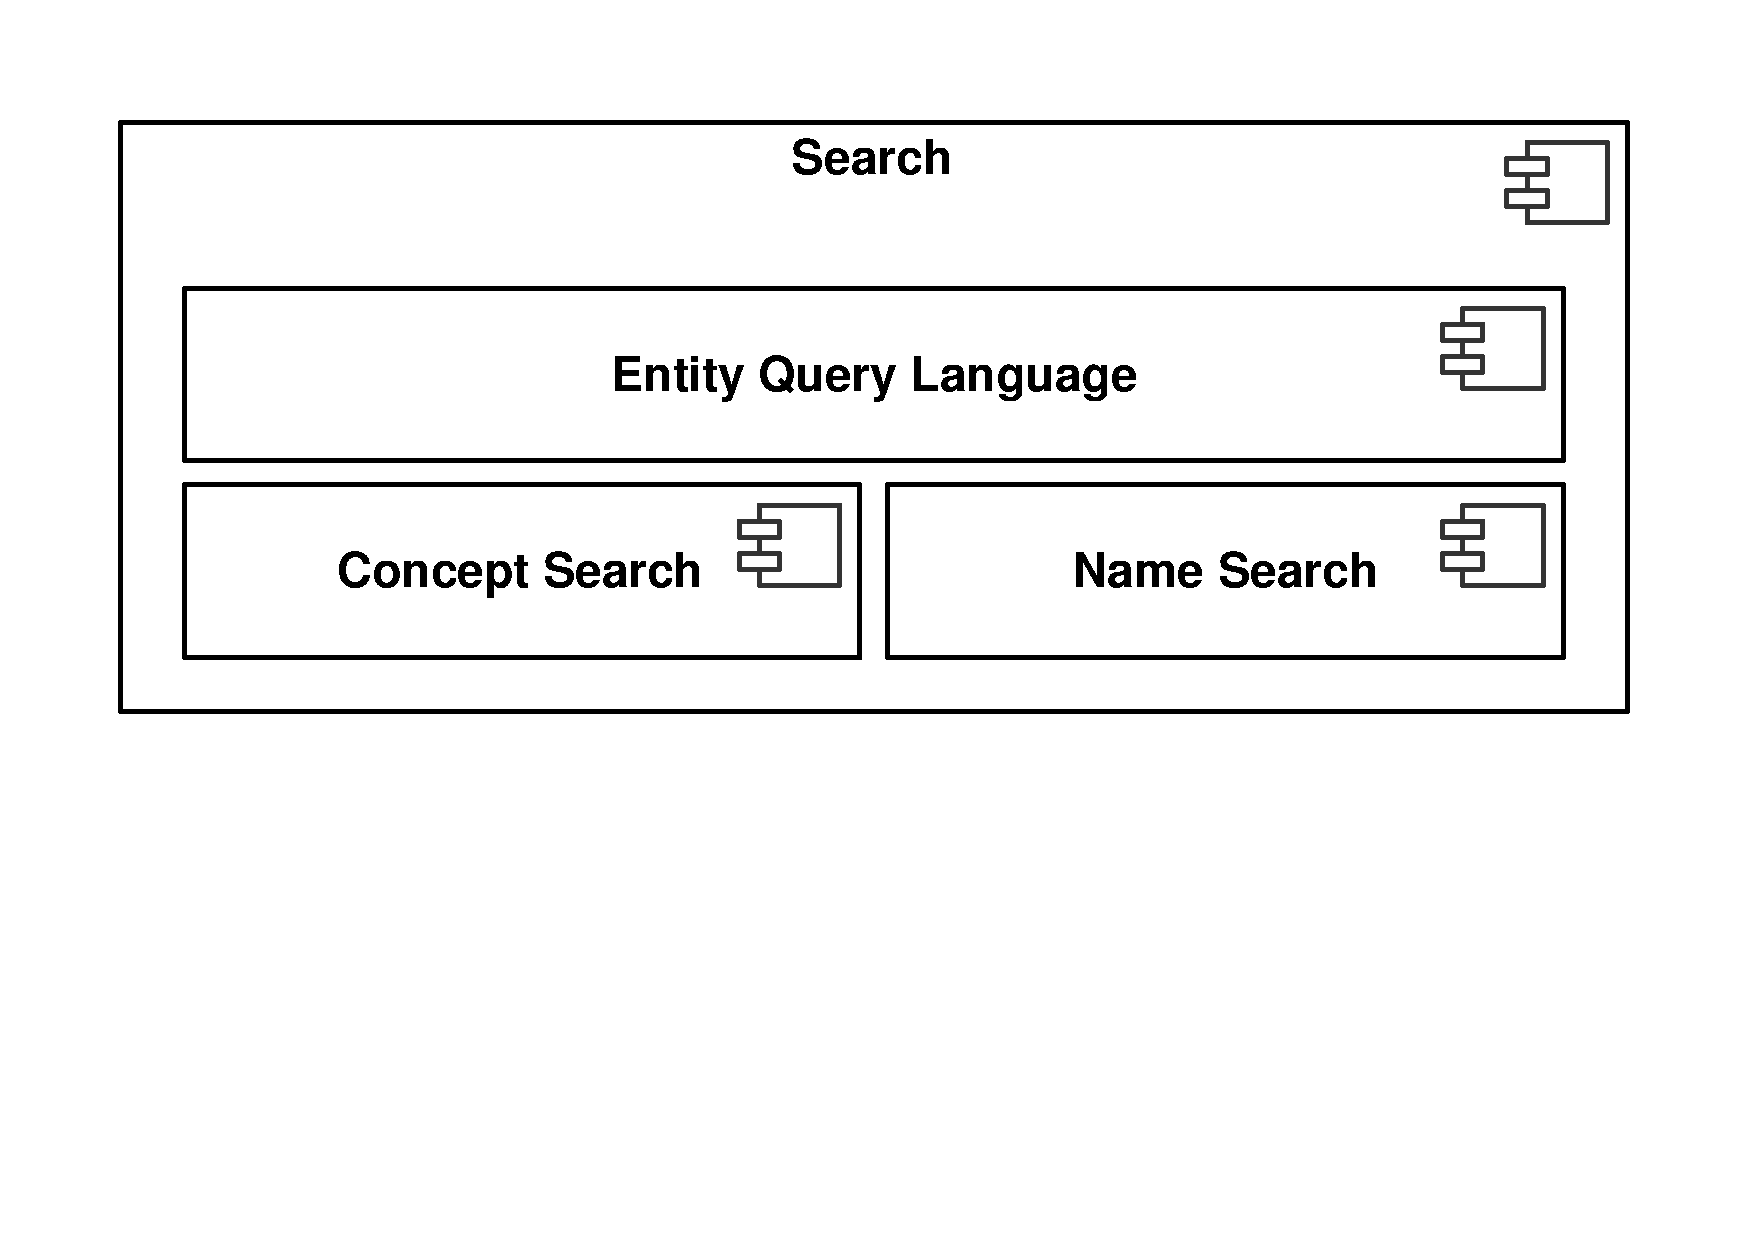
\includegraphics[width=0.65\textwidth]{figures/SearchComponentDiagram}
\caption{Search Diagram}
\label{fig:search_diagram}
\end{figure}

\paragraph{Concept Search.} 
\label{par:concept_search}
The lower part of Fig.~\ref{fig:search_diagram} shows two approaches that are used to deal with descriptions and names of peers. In particular, Concept Search, is used to match attributes from peers profiles with the search request. Concept Search~\cite{Giunchiglia:2009fk} was inspired by many syntactic IR systems that implement term matching by computing string similarity between words. For example, search for identical (possibly stemmed) words, words with common prefixes, words within a certain edit distance with a given word, or words that sound similar (see~\cite{Manning:2008:IIR:1394399} for more details on existing syntactic search approaches). 

However, when trying to match peer's attributes with a search query in the PM, there are many problems related with syntactic IR systems that can negatively affect the quality of search results. In particular, we know that different words can have the same meaning (synonymy); the same word may have multiple meanings (polysemy); and the meaning of words can be different but still semantically related. To deal with these problems, Concept Search extends the syntactic search approach with semantic search. In this approach, the retrieval models and data structures of syntactic search are reused. The main difference is given by the fact that concept search leverages on the core semantic data model of the PM and therefore concepts are used as terms instead of words. As a consequence, term matching is implemented by using semantic matching of concepts~\cite{Giunchiglia:2007ve}. On the other hand, when the semantic information is not available (i.e., when the concepts of a given set of words cannot be computed), words are used as terms and concept search falls back to the underlying syntactic search.


\paragraph{Name Search.} 
\label{par:name_search}
When dealing with peers that can be humans, it is important to account for the relevance of human readable identifiers (i.e., names). 
Names are labels composed by a combination of words, numbers and symbols. They are different from other attributes because they play the role of keywords rather than been mapped to concepts from a knowledge base. 
A name search algorithm deals with the problem of finding all the possible candidate entities that have names equal or similar to a given name.

Names can suffer from different types of variations, such as, format variations (e.g., \emph{George Augusto Lombardi} vs. \emph{George A. Lombardi} vs. \emph{Lombardi, George}), translations (e.g., \emph{Trento} in Italian vs. \emph{Trient} in German vs. \emph{Trent} in English), or misspellings (e.g., \emph{Fausot} vs. \emph{Fausto} vs. \emph{Fuasot}). These name variations show the complexity with which a name search algorithm has to deal. Various syntactic search techniques can be used for implementing name search. 

In the name search algorithm implemented by the PM, the following techniques are applied in a sequential order until the entities with the matching names are found:
\begin{inparaenum}[(i)]
\item \emph{Exact matching} between a given name and the entity name; 
\item \emph{Fuzzy search} techniques are employed by comparing name tokens using, for instance, jaccard~\cite{Bilenko:2003pd} similarity coefficient for comparing the similarity\footnote{\url{http://en.wikipedia.org/wiki/Similarity_measure}} of token sets.
\item Prefix search technique is used to perform fuzzy search on tokens themselves to account for the fact that, according to~\cite{Pollock:1984rr}, fewer errors usually occur at the beginning of names. 
%Search for name tokens having the same prefix can be efficiently implemented both in the inverted index vocabulary and by using SQL like queries.
\item Finally, the trigram search technique (N-gram index with grams of length 3) is used to account for the case of misspelled names. The pg\_trgm\footnote{\url{http://www.postgresql.org/docs/8.4/static/pgtrgm.html}}  module from PostgreSQL database management systems is used to implement trigram search on entity names in the current implementation. 
\end{inparaenum}


\paragraph{Entity Query Language.} 
\label{par:entity_query_language}
The upper part of the figure shows a subcomponent that builds on the two types of searches presented above and supports additional search operations based on the relations between entities. An Entity Query Language (EQL) provides more flexible and heterogeneous language to access peer’s attributes as well as additional operations. 
EQL is used by the PM to extend the low-level mechanisms. It can be seen as a semantically enabled version of HQL\footnote{\url{http://docs.jboss.org/hibernate/core/3.3/reference/en/html/queryhql.html}} on entities, where HQL is an object-oriented query language similar to SQL. More details about EQL are provided in the Annex~\ref{sec:search-annex}.


\subsection{Implementation}
%\todo{how it has been implemented} 

The Peer Manager's implementation of its search service (search, matching and ranking services) uses Java in combination with Hibernate and Spring frameworks, a PostgreSQL database is used for storage of peers' information and profiles. The Peer Manager front-end uses NodeJs and exposes its basic search functionalities through a low level HTTP API. In order to facilitate the interaction with other SmartSociety components (also in light of specific prototypes and demos), the PM provides also a high level API that results in more powerful and easy-to-use calls. Such calls leverage the full power of the Peer Manager and allow other components to abstract from internal details related to the PM's implementation. 

It is important to note that the implementation of the underlying mechanisms at the core of the PM's search implementation represent previous knowledge/work of the University of Trento Knowdive research group, so its source code will not be made commonly available. However, the full source code of the high level API corresponding to the front-end implementation that is specific for SmartSociety will be made available as part of the project. In the rest of this section we provide more details on how to use the search service, which in turn is related with the implementation of the high level API. 

\subsubsection{Search Service}\label{subsec:concept_search}
%\todo{documentation of search service including syntax/examples of EQL}

The Concept Search approach is used by the PM to implement concept based search on attributes from peers profiles.
The syntax of attribute-based concept search queries is designed to be similar to the query syntax of Lucene\footnote{\url{http://lucene.apache.org/core/old_versioned_docs/versions/3_5_0/queryparsersyntax.html}}, a popular Java based open-source indexing and search library. The current implementation supports concept search on attribute values, e.g. the query \emph{``big restaurant''} among other results will also return entities with attributes containing phrase \emph{``huge steakhouse''}. Concept search is also implemented on top of attribute names, e.g. the entity with attribute \emph{``location:Trento''} will be returned as an answer to query \emph{``place:Trento''}. Atomic queries on attribute values and attribute names can be combined into more complex queries by using Boolean operators, e.g. \emph{``big restaurant AND location:Trento''}.

The more flexible access to search services can be exploited through the specification of a search query using EQL language. The current implementation of the PM's search service supports only a subset of HQL, however, new features will be added if (and when) needed. The EQL implementation currently used in the PM supports the FROM clause, allowing the simplest query specification, as well as the SELECT, JOIN, GROUP BY, WHERE, and ORDER BY clauses that allow the specification of more complex queries. Among them, the ORDER BY clause is of key importance because is the one that is used to implement the ranking of search results. 

Note that concept search is used within FROM and SELECT clauses, which means that there is no need to know the exact name of the entity type or attribute name. Concept search approach is used for matching entity types in \emph{from} clauses and attribute names in \emph{select} clauses. 
 For instance, in the case when there is a synonymy relationship between concepts \emph{restaurant} and \emph{bar} in the underlying knowledge base, the search to find all the restaurants can also be performed by using the query ``\texttt{FROM bar r}''.

Another use of concept search query in \emph{from} clause can be to select a subset of all the entities for a given entity type. 
This is done by adding additional constraints, using concept search syntax, into the \emph{from} clause.
For instance, in the query ``\texttt{FROM bar [description:steakhouse] r}'', the additional constraint ``\texttt{[description:steakhouse]}'' requires that descriptions of found bar entities contain concepts which are more specific than the concept `steakhouse'. This means that a description containing `steakhouse in Trento' would comply with such requirement and the corresponding entity can be included in the search result. 
%\todo{Last sentence unclear, please clarify example}


%%%%%%%%%%%%%%%%%%%%%%%%%%
%%%%%%%%%%-Limitations-%%%%%%%%%%
%%%%%%%%%%%%%%%%%%%%%%%%%%

%On the other hand, the current limitations include:
%\begin{enumerate}
%\item \textbf{Joins:} Only inner join is supported, i.e., the keyword \emph{join} is used for specifying inner join.
%\item \textbf{Nulls:} If an attribute name is selected, then only NOT NULL attribute values will be returned.
%
%\begin{tabular}{ll}
%\texttt{SELECT cat FROM Cat cat} & [all cats will be found] \\
%\texttt{SELECT cat, cat.name FROM Cat cat} & [cats without names will be skipped] \\
%\end{tabular}
%\item \textbf{Aggregates:} Only simple aggregate functions on attributes are supported, e.g. count(cat).
%\item \textbf{Dots:} As in HQL, dot-notation is used for accessing entity attributes. There are limitations on how dots are used. The first (and only the first) dot defines an attribute (e.g. cat.name). The second dot can be used only for accessing the meta-data (e.g. cat.name.metadata). Note, that it is not really a limitation because all the queries with two or more dots can be rewritten by using explicit joins, as it is shown below:
%
%\begin{tabular}{p{0.45\textwidth}p{0.45\textwidth}}
%\texttt{SELECT cat.mate.name} & [not supported] \\
%\texttt{FROM Cat cat} & \\
% & \\
%\texttt{SELECT mate.name}  & [equivalent query with explicit join] \\
%\texttt{FROM Cat cat} & \\
%\texttt{JOIN cat.mate mate} & \\
%\end{tabular}
%\end{enumerate}


%%%%%%%%%%%%%%%%%%%%%%%%%%
%%%%%%%%%%-Additional notes-%%%%%%%
%%%%%%%%%%%%%%%%%%%%%%%%%%

%Additional notes:
%\begin{itemize}
%\item If no attribute is specified in select or where clause, entity id is used as a default attribute. For instance, 
%``\texttt{SELECT cat FROM Cat cat}'' internally, will be translated to ``\texttt{SELECT cat.id FROM Cat cat}''
%
%\item Specifying an alias (e.g. cat) is required. For instance, ``\texttt{FROM Cat cat}''
%
%\item If concepts with multi-words are used for defining types or attributes, spaces between words should be replaced with underscore `\_'. For instance, ``\texttt{SELECT cat.first\_name FROM Cat cat}''.
%
%\item Underscore `\_' can also be used for specifying correct concepts which should be used for attribute names and types. For instance, ``\texttt{SELECT cat.name\_123 FROM Cat\_321 cat}''.
%\end{itemize}
%


\subsubsection{Main Search Endpoint Documentation}
%\todo{The specification of the search APIs with an example will be added here for the final version of this document.}

The Table~\ref{tab:searchApi} shows the specification of the search API and a simple example of the call and response for searching all available peers for a generic task. 

\begin{table}[htdp]
\caption{Search API}
\begin{center}

\begin{tabular}{|l|l|p{9cm}|}
\hline
\textbf{Method} & \textbf{Api} & \textbf{Description} \\
\hline
GET & 
instances/search & 
Returns a set of entity instances that match with the characteristics specified in the input query. In the example, the call is used to obtain a list of users representing peers that matches with a set of requirement. \\
\hline
\multicolumn{3}{|c|}{\textbf{Call Example}} \\
\hline
\multicolumn{3}{|p{14cm}|}{
\url{
http://demos.disi.unitn.it:8080/smartsociety-score-api/instances/search?query=select\%20user1\%20from\%20User\%20user1\%20join\%20user1.entity\%20person1\%20where\%20person1.available\%20\%3D\%20true\&entityBase=5408\&instanceClass=Instance\&queryType=\%20EQL\&parseSemantics=false\&includeExplanation=false\&includeCount=false\&idsOnly=false\&pageIndex=1\&pageSize=10\&maxDepth=1\&includeSemantics=false\&maxValues=10\&includeAttributes=false\&createAttributeMap=false\&attributeFilterType=ATTRIBUTE\_DEF\_ID\&includeAttributesAsProperties=false\&includeTimestamps=false
}}
\\ 
\hline
\multicolumn{3}{|c|}{\textbf{Response Example}} \\
\hline
\multicolumn{3}{|p{14cm}|}{
\{
  ``@type'': ``EQLSearchResult'',
  ``results'': [
      [``6604''],
      [``6605''],
      [``6606'']
  ]
\}
} \\
\hline
\multicolumn{3}{|c|}{\textbf{Response General}} \\
\hline
\multicolumn{3}{|p{14cm}|}{
\{
  ``@type'': ``EQLSearchResult'',
  ``results'': [
      [``\textcolor{ao(english)}{$\langle$ Returned userId 1$\rangle$}''],
      \textcolor{ao(english)}{\ldots}
      [``\textcolor{ao(english)}{$\langle$ Returned userId N$\rangle$}'']
  ]
\}
} \\
\hline


%\multicolumn{3}{|l|}{\{} \\
%\multicolumn{2}{|l}{``@type'': ``EQLSearchResult'',} & \\
%\multicolumn{2}{|l}{``results'': [ } \\
%\multicolumn{3}{|l|}{ [``6604''],} \\
%\multicolumn{3}{|l|}{ [``6605''],} \\
%\multicolumn{3}{|l|}{ [``6606''] } \\
%\multicolumn{3}{|l|}{ ] }\\
%\multicolumn{3}{|l|}{\}} \\
%\hline
\end{tabular}

\end{center}
\label{tab:searchApi}
\end{table}%





















\section{Privacy-preserving Measures}
{\it here goes all discussion on how the current implementation supports privacy, what is missing and when -and if- it will be delivered}
 
\todo{this section could be removed because the privacy preserving measures are embedded in sections \ref{sec:profiling} and \ref{sec:matching_ranking}}

\section{Evaluation}
\label{sec:evaluation}
%\todo{RONALD and ALETHIA}

%{\it including assessment against functional requirements - elicited from use cases - and performance measures based on the actual  deployment}
  
  
\todo{this section contains preliminary content}

%Intro to evaluation
\todo{missing section introduction}
%Privacy and security as a second concern

\subsection{Analytic Validations}
The analytic part of the validation include formal or semi-formal validations and analysis of the different properties of the system. This validation tests will be interested, in particular, in comparing the implemented version of the Peer Manager with its ideal counterpart described during the first and second year deliverables (requirement compliance) and also finding out ``the cost of privacy'' by calculating the overhead in time and space that implementing these privacy measures brings to general systems.

The first results of this analytic validation activities will be reported during the third year review meeting of the project with the final results reported in D4.4 and the fourth year review meeting.

\subsubsection{Requirement compliance}
The requirement compliance of the peer manager comprises both evaluation of the general project requirements (found in the DoW and in D1.1??) and the compliance with the privacy requirements established in D4.1 and revised in D4.2.

For the compliance with the privacy requirements we plan to express a simplified version of the Peer Manager using the formalization of privacy sensitive systems found in [??]. We will then proceed to prove the extent to which the so represented Peer Manager is in fact compliant with the privacy requirements set in earlier version of this deliverable. 

The strategy for validation of the project requirements will include applied methods such as unit and integration tests of the Peer Manager implementation; along with performance tests of the integrate Peer Manager as part of the project's use cases. For the last case, performance evaluations in both time and space will also be performed and reported accordingly.  

\subsubsection{``Cost of privacy'' measurements}
This exercise will compare the time and space complexity of two Peer Managers, one without any privacy considerations and the other (as developed for the project) compliant with the set privacy requirements. Generalizing one step further, it is expected that this comparison would be able to show an estimate of the cost in time and space complexity for complying with these privacy requirements (that are now part or being discussed to become part of the EU privacy legislation) in a wide-range of relevant systems.

More in particular, the time/space complexity in both the privacy-less and the privacy-enabled Peer Managers will be compared independently for storing information and reading/accessing this information, 

\subsection{SmartShare Exploratory Survey}
SmartShare is a ridesharing application developed by the SmartSociety consortium as test and validation of several of the project's ideas.  A trial using the SmartShare application is planned during the second half of 2015 in multiple Italian municipalities.  

As part of the SmartShare trial, we plan to carry out an exploratory survey aimed initially to gauge the interest and knowledge of the participating users in privacy-related issues and technologies. Furthermore, based on these results we plan to adjust and create requirements related to the focused user activities and testing planned for year four.
 
The list of the questions being asked in this exploratory survey can be found in the Appendix~\ref{sec:smartshare-survey} and the results of this validation activity will be reported during the third year review of the project.

\subsection{Usage analysis of the SmartSociety Platform}
Through integration with the SmartSociety platform the peer manager will be used in several of the small-scale experiments organized by WP8 and also the Virtual Gamified Environment developed as part of WP9. We will take these opportunities to measure the real-use performance of the Peer Manager and, when possible, get information from the involved users.

\todo{Specific questions to be asked by WP4 towards the Virtual Gamified Environment to be added here}

The results of this validation activity will be part of the D4.4 and will be reported during the fourth year review of the project.

\subsection{Focused user activities and testing}
The final focused user activities relating to the peer manager and platform-wide privacy considerations will be carried out during the fourth year of the project. We plan to use all previous validations (specially the SmartShare Exploratory Survey) to inform and better adjust this validation activity. 

Based on this, further quantitative and qualitative user-related studies may be carried out, already aiming to validate not only the Peer Manager but also to draw project-wide and CAS-related conclusions of the exercise. 

The results of this validation activity will be part of the D4.4 and will be reported during the fourth year review of the project.


\section{Integration}
\label{sec:integration}
The Peer Manager has been integrated in the SmartSociety platform
during the second year of the project, and released as component of
the version 1.0 of the platform. 

Currently the Peer Manager functionality
is used in both project-wide scenarios, i.e., SmartShare and
AskSmartSociety!~\cite{D8.2,D8.3}.

In general terms, the PM is mostly used as privacy-preserving
information service for peer-related information. In this sense, it is
at the center of a rather complex web of interactions with other
components. In particular, it is used by the Orchestration Manager to
identify suitable peers for carrying out a given task (composition
phase). It also provides information on how peers shall be contacted
for the negotiation process, the actual interaction being mediated by
the SmartCom middleware. The PM is tightly interacting with the
Context Manager, a component (developed within WP3) able to mine
streams of data to provide a near real-time representation of the
current user context. This situational information is integrated as
dynamic part of the user profile, and can be used for ensuring the
search process returns purposeful results. 

In this section we briefly describe how the PM is used in the context
of overall SmartSociety platform architecture, with reference to the
two aforementioned scenarios.

In both contexts, the PM is used to perform all operations related to
the management of collectives
(creation, retrieval of peers in a collective and retrieval of peer
information and contact method for communication
purposes~\cite{D8.2}). In SmartShare a collective is the set of peers
representing users taking part in a ride. In AskSmartSociety! a
collective is the set of peers selected as adequate (by the PM) to
answer a given question. These operations are typically requested by
the application peer (creation of collective) and by the SmartCom
communication middleware (retrieval of peers in a collective and peer information).

The PM search functionality plays a key role in the AskSmartSociety!
application scenario, where it is exploited to identify a suitable set
of peers who could best contribute to answer a given
question. This function is invoked by the OM and the response triggers
the execution of the negotiation process~\cite{D8.2}. In the context
of AskSmartSociety!, the ability of
the PM to handle transparently machine and human peers represent a key
feature, in that it enables full hybridity of the application. Also, the usage of the Concept Search approach, and in
particular the ability of the PM to perform semantic matching on
peers' attributes is instrumental in identifying human peers with the
right expertise to answer a given query, hence contributing
significantly to the quality of the answers collected.


\section{Conclusions}
\label{sec:concl}
This deliverable included the description of  a number of key aspects related to the PM design, implementation and validation. 
In particular, it included:
\begin{itemize}
\item The mechanisms and implementation details for the profile schemas and the privacy-enhancing technologies used by the PM;
\item The mechanisms and implementation details for the services that allow searching, matching and ranking of peers based on different attributes (i.e., characteristics) from their profiles;
\item The evaluation plans for the PM including analytical and user-based evaluations; and
\item The description of how the PM is currently integrated in the SmartSociety platform and used in different project-wide scenarios.
\end{itemize}
In the second half of 2015 the focus will be on the validation of the PM functionality and performance, following the strategy outlined in Sec.~\ref{sec:integration}. At the same time, feedback from empirical activities in WP8 and WP9 will be used to fine-tune the PM APIs and the underlying mechanisms, with particular emphasis on search and ranking functionality. The final PM design and implementation will be shipped with D4.4 at M42.

%%%%%%%%%%%%%%%%%%%%%%%%%%%%%%%%%%%%%%%%%%%%%%%%%%%%%%%%%%%%%%
\newpage

%%%%%%%%%%%%%%%%%%%%%%%%%%%%%%%%%%%%%%%%
%%%%%%%%%%%%%%%%%%%%%%%%%%%%%%%%%%%%%%%%%%%%%%%%%%%%%%%%%%%%%%%%%%%%%%%%%%%%%%%%%%%%%%%%%%%%%%%%%%%%%%%%%%%%%%%%%%%%%%%%
\bibliographystyle{./IEEEtran}
\bibliography{BIB/biblio.bib}
%\clearpage
%\appendix
%\section{Details on code}
%\input{sections/annex1}
\end{document}
